\documentclass[a4paper, 11pt, titlepage]{article}
\usepackage{fancyhdr}
\usepackage{graphicx}
\usepackage{imakeidx}
\usepackage{makeidx}
\usepackage{mathtools}
\usepackage[spanish]{babel}
\usepackage{eurosym}
\usepackage{hyperref}
\usepackage{amssymb}
\usepackage{listings}
\usepackage{xcolor}

% \setcounter{secnumdepth}{5}
% \setcounter{tocdepth}{5}

\title{{\scshape\Huge Sistemas Operativos Distribuidos \par}}
\author{Francisco Javier Balón Aguilar}

\begin{document}
\maketitle
\renewcommand{\contentsname}{Índice de contenidos} % Nombre dado al ?ndice
\tableofcontents % Genera la tabla de contenidos del ?ndice autom?ticamente
%\newpage

%Lista de figuras 
\listoffigures
%\newpage

%Lista de tablas 
\listoftables
\newpage

\section{Introducción}

    \subsection{Estructura de un sistema distribuido}

        \subsubsection{Funciones de un sistema distribuido}

        \subsubsection{Características de un sistema distribuido}

    \subsection{Tipos de sistemas operativos distribuidos}

\section{Sistemas operativos multiprocesador}

    \subsection{Arquitectura de un sistema operativo multiprocesador}

        Los equipos que cuentan con más de un procesador y que comparten la misma memoria
        se denominan sistemas multiprocesador. En ellos, debe existir un sistema operativo 
        común y central, que controle las operaciones de cada procesador, así como su 
        gestión, coordinación y accesos a memoria.

        Este tipo de sistemas proporcionan una mayor productividad del sistema, ya que 
        pueden realizar un mayor número de tareas en un menor espacio de tiempo, y una 
        mayor velocidad de aplicación, ya que al aumentarse el número de procesadores,
        disminuye el tiempo de espera de un proceso para ser procesado.

        Estos sistemas ofrecen una serie de ventajas:

        \begin{itemize}
            \item \textbf{Rendimiento y potencia de cálculo}.
            \item \textbf{Tolerancia a fallos}.
            \item \textbf{Flexibilidad}.
            \item \textbf{Relación coste/rendimiento}.
        \end{itemize}

        Podemos clasificar los sistemas multiprocesador según el modo de trabajo en:

        \subsubsection{Procesamiento asimétrico}

            El procesamiento asimétrico\footnote{
                El modo de procesamiento asimétrico se originó en 1970 en el Instituto
                 Tecnológico de Massachusetts (M.I.T.). 
            } entre varios ordenadores permite ejecutar procesos 
            de manera independiente separados del procesador que controla y tiene instalado
            el sistema operativo.\footnote{
                A día de hoy este modo de procesamiento no se utiliza casi salvo en 
                aplicaciones muy concretas como puede ser la PS3 de Sony, donde el 
                procesador central tiene sub-procesadores que se encargan de tareas 
                muy específicas.
            }

            Aunque a nivel físico ya no se utilice este diseño de arquitectura, a nivel 
            lógico si que se sigue implantando en sistemas donde cada procesador se encarga
            de una tarea específica, por ejemplo, un procesador puede ser el responsable
            de las operaciones de disco, otro de las operaciones de video, etc. Estos
            sistemas no tienen la flexibilidad de asignación de tareas a los procesadores 
            menos cargados, estando predefinidas por defecto.

            \begin{figure}[htp]
                \centering
                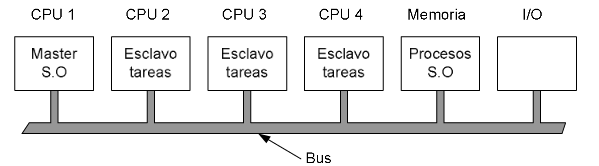
\includegraphics[width=1\textwidth]{resources/multiprocesador_asimetrico.png}
                \caption{Representación de multiprocesador asimétrico}
                \label{multiprocesador_asimetrico}
            \end{figure}

        \subsubsection{Procesamiento simétrico}

            En un sistema multiproceso, cada uno de los procesadores deben ser equivalentes,
            con funciones similares, aunque haya alguno que realice tareas específicas.

            A nivel de hardware, en los sistemas simétricos cada procesador puede acceder a 
            la memoria RAM por completo. Cada procesador tiene la misma importancia a la hora
            de acceder, por lo tanto todas las CPUs pueden interaccionar y compartir memoria 
            entre ellas.
            
            A nivel de software, e independientemente del sistema operativo que lo gestione, 
            cada procesador tiene capacidad para enviar o repartir tareas a otros procesadores. 
            Al no existir una unidad central, y tener acceso total a la memoria, cada procesador 
            es capaz de terminar cualquiera de las tareas asignadas. \footnote{
                Al ser todos los procesadores idénticos, ante el fallo de uno de ellos el sistema 
                operativo lo retira y lo notifica al operador. Todos los procesadores pueden cooperar
                en la ejecución de un mismo proceso. Aun así, esta arquitectura también puede producir 
                largas colas de espera.
            }

            \begin{figure}[htp]
                \centering
                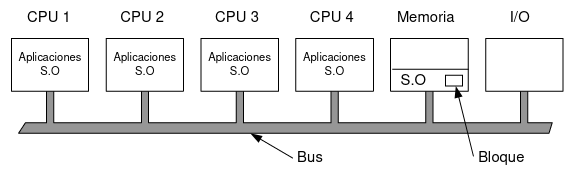
\includegraphics[width=1\textwidth]{resources/multiprocesador_simetrico.png}
                \caption{Representación de multiprocesador simétrico}
                \label{multiprocesador_simetrico}
            \end{figure}


        \subsubsection{Interconexión de los procesadores}

    \subsection{Gestión del procesador}

        \subsubsection{Asignación de los procesadores}

        \subsubsection{Planificación del procesador}

    \subsection{Sincronización y gestión de la memoria}

        \subsubsection{Algoritmos de sincronización}

% BIBLIOGRAFÍA Y REFERENCIAS
\newpage
\begin{thebibliography}{X}
    \bibitem{} Desarrollo de un sistema expertocon lógica difusa, Jorge Franco Herrera y Angélica Franco Arias \\ \url{https://ingsistycomp.files.wordpress.com/2017/09/proyecto-1-sistema-experto-difuso.pdf}
    \bibitem{} Diseño de un Sistema Experto Difuso para la Determinación de la Densidad de Corriente en una Planta de Cromado, Carolina V. Ponce y Bayron Rojas \\ \url{https://scielo.conicyt.cl/scielo.php?script=sci_arttext&pid=S0718-07642019000200157}
    \bibitem{} Modelo basado en Lógica Difusa para el Diagnóstico Cognitivo del Estudiante \\ \url{https://scielo.conicyt.cl/scielo.php?script=sci_arttext&pid=S0718-50062012000100003}
    \bibitem{} Sistemas Expertos y Lógica Difusa \\ \url{http://catarina.udlap.mx/u_dl_a/tales/documentos/lmt/maza_c_ac/capitulo2.pdf}
    \bibitem{} Sistema de Control Difuso para Unidades de Cuidados Intensivos (UCI), Jefferson Steven Soto Medellín \\ \url{https://repository.ucatolica.edu.co/bitstream/10983/1278/1/Sistemas%20de%20Control%20Difuso%20para%20Unidades%20de%20Cuidado%20Intensivo%20(Trabajo%20Final)%20701429%20Nuevo.pdf}
\end{thebibliography}

\end{document}
